\section{Temporal Difference algorithms}
\label{sec:TD}


%In this lecture we will continue looking at model-free learning. In
%the previous lecture we presented: (1) $Q$-learning, which is an
%off-policy learning algorithm that learns the optimal $Q^*$
%function, (2) {\tt SARSA} which is an on-policy variant of
%$Q$-learning where we need to select actions, and (3) Monte-Carlo
%which is a model-free algorithm to learn the value function from
%episodes.

In this section we will look on temporal differences methods, which
works in an online fashion. We will start with $TD(0)$ which uses
only the most recent observations for the updates, and we will
continue with methods that allow for a longer look-ahead, and then
consider $TD(\lambda)$ which averages multiple look-ahead
estimations.

In general, temporal differences (TD) methods, learn directly from
experience, and therefore are model-free methods. Unlike Monte-Carlo
algorithms, they will use incomplete episodes for the updates, and
they are not restricted to episodic MDPs. The TD methods update
their estimates given the current observation and in that direction,
similar in spirit to $Q$-learning and SARSA.

\subsection{TD(0)}

Fix a policy $\policy\in \Pi_{SD}$, stationary and deterministic. The goal
is to learn the value function $\Value^\policy(\state)$ for every
$s\in S$. (The same goal as Monte-Carlo learning.) The TD algorithms
will maintain an estimate of the value function of the policy
$\policy$, i.e., maintain an estimate $\widehat{V}_\ttime(\state)$
for $\Value^\policy(\state)$. The TD algorithms will use their
estimates $\widehat{V}$ for the updates. This implies that unlike
Monte-Carlo, there will be an interaction between the estimates of
different states and at different times.

As a starting point, we can recall the {\em value iteration}
algorithm.
\[
V_{\ttime+1}(\state)=E^\policy[\reward(\state,\policy(\state))+\discount
V_\ttime(\state')]
\]
We have shown that value iteration converges, namely $V_\ttime
\rightarrow_{\ttime\rightarrow\infty} \Value^\policy$.

Assume we sample
$(\state_\ttime,\action_\ttime,\reward_\ttime,\state_{\ttime+1})$.
%Assume that $\policy\in SD$, namely a stationary deterministic policy.
Let $\widehat{V}_\ttime$ our estimation at time $\ttime$,
and we sample
$(\state_\ttime,\action_\ttime,\reward_\ttime,\state_{\ttime+1})$.
Then,
\[
E^\policy[\widehat{V}_\ttime(\state_\ttime)]=
E^\policy[\reward_\ttime+\discount
\widehat{V}_\ttime(\state_{\ttime+1})]=E^\policy[\reward(\state,\action)+\discount
\widehat{V}_\ttime(\state')|\state=\state_\ttime,a=\policy(\state)]
\]
%where $E^\policy [\widehat{V}_\ttime]=V_\ttime$.

The $TD(0)$ will do an update in this direction, namely,
$[\reward_\ttime+\discount \widehat{V}_\ttime(\state_{\ttime+1})]$.

\paragraph{$TD(0)$ Algorithm}

\begin{itemize}
\item \emph{Initialize:} $\widehat{V}(\state)$ arbitrarily.

\item At time $\ttime=0,1,\dots$:


-- Observe: $(\state_\ttime, \action_\ttime, \reward_\ttime,
\state_{\ttime+1})$.

-- Update:
%$(\state_\ttime,\action_\ttime,\reward_\ttime,\state_{\ttime+1})$:
\[
\widehat{V}(\state_\ttime)=\widehat{V}(\state_\ttime)+\alpha_\ttime(\state_\ttime,\action_\ttime)
\big[\reward_\ttime+\discount
\widehat{V}(\state_{\ttime+1})-\widehat{V}(\state_\ttime)\big]
\]
where $\alpha_\ttime(\state,\action)$ is the step size for
$(\state,\action)$ at time $\ttime$.
\end{itemize}

We define the {\em temporal difference} to be
\[
\Delta_\ttime =\reward_\ttime+\discount
\widehat{V}(\state_{\ttime+1})-\widehat{V}(\state_\ttime)
\]
The $TD(0)$ update becomes:
\[
\widehat{V}(\state_\ttime)=\widehat{V}(\state_\ttime)+\alpha_\ttime(\state_\ttime,\action_\ttime)\Delta_\ttime
\]


[[YM: motivating example. Waze?!]]

We would like to compare the $TD(0)$ and the Monte-Carlo (MC)
algorithms. Here is a simple example with four states
$S=\{A,B,C,D\}$ where $\{C,D\}$ are terminal states and in $\{A,B\}$
there is one action (essentially, the policy selects a unique
action). Assume we observe eight episodes. One episode is
$(A,0,B,0,C)$, one episode $(B,0,C)$, and six episodes $(B,1,D)$. We
would like to estimate the value function of the non-terminal
states. For $V(B)$ both $TD(0)$ and $MC$ will give $6/8=0.75$. The
interesting question would be: what is the estimate for $A$? MC will
average only the trajectories that include $A$ and will get $0$
(only one trajectory which gives $0$ reward). The $TD(0)$ will
consider the value from $B$ as well, and will give an estimate of
$0.75$. (Assume that the $TD(0)$ continuously updates using the same
episodes until it converges.)

We would like to better understand the above example. For the above
example the empirical MDP will have a transition from $A$ to $B$,
with probability $1$ and reward $0$, from $B$ we will have a
transition to $C$ with probability $0.25$ and reward $0$ and a
transition to $D$ with probability $0.75$ and reward $1$. (See,
Figure~\ref{fig:L7-ML}.) The value of $A$ in the empirical model is
$0.75$. In this case the empirical model agrees with the $TD(0)$
estimate, we show that this holds in general.


\begin{figure}
  % Requires \usepackage{graphicx}
  \begin{centering}
  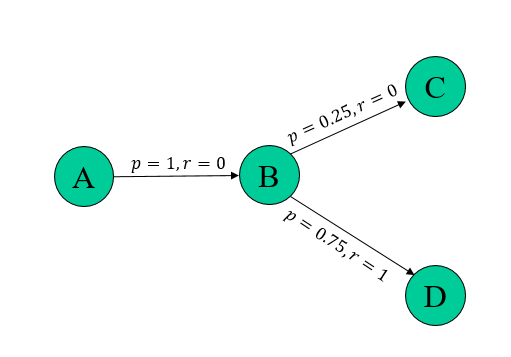
\includegraphics[width=0.5\textwidth]{figures/L7-ML}\\
  \caption{The situated agent}\label{fig:L7-ML}
  \end{centering}
\end{figure}


\paragraph{Maximum Likelihood model}\footnote{YM: repeat} Recall that the empirical model, which is also the
maximum likelihood model, of a sample be define as follows. Let
$n(\state,\action)$ be the number of times $(\state,\action)$
appears in the sample. Given a sample
$(\state_\ttime,\action_\ttime,\reward_\ttime,\state_{\ttime+1})$
for $1\leq t\leq T$, we define the empirical model as follows. The
rewards $\widehat{\reward}(\state,\action)$ are the average rewards
of $(\state,\action)$, i.e.,
$\widehat{\reward}(\state,\action)=\frac{1}{n(\state,\action)}\sum_{\ttime:\state_\ttime=\state,\action_\ttime=\action}\reward_\ttime$
and
$\widehat{p}(\state'|\state,\action)=\frac{n(\state,\action,\state')}{n(\state,\action)}$,
where $n(\state,\action,\state')$ is the number of samples that have
$\state_{\ttime+1}=\state'$ when $\state_\ttime=\state$ and
$\action_\ttime =\action$.

The following theorem states that the value of $\policy$ on the
empirical model is identical to that of $TD(0)$ (running on the
sample until convergence, namely, continuously sampling uniformly
$t\in[1,T]$ and using $(\state_\ttime,
\action_r,\reward_\ttime,\state_{\ttime+1})$ for the $TD(0)$
update).

\begin{theorem}
Let $\Value^\policy_{TD}$ be the estimated value function of
$\policy$ when we run $TD(0)$ until convergence. Let
$\Value^\policy_{EM}$ be the value function of $\policy$ on the
empirical model. Then, $\Value^\policy_{TD}=\Value^\policy_{EM}$.
\end{theorem}

\begin{proof}[Proof sketch]
The update of $TD(0)$ is
$\widehat{V}(\state_\ttime)=\widehat{V}(\state_\ttime)+\alpha_\ttime(\state_\ttime,\action_\ttime)\Delta_\ttime$,
where $\Delta_\ttime=\reward_\ttime+\discount
\widehat{V}(\state_{\ttime+1})-\widehat{V}(\state_\ttime)$. At
convergence we have $E[\Delta_\ttime]=0$ and hence,
\[
\widehat{V}(\state)=\frac{1}{n(\state,\action)}\sum_{\state_{\ttime+1}:\state_\ttime=\state,\action_\ttime=\action}
\reward_\ttime+\discount
\widehat{V}(\state_{\ttime+1})=\widehat{\reward}(\state,\action)+\discount
E_{\state'\sim
\widehat{p}(\cdot|\state,\action)}[\widehat{V}(\state')]
\]
where $\action=\policy(\state)$.
\end{proof}

In is worth to compare the above theorem to the case of Monte Carlo
(Theorem~\ref{thm:MC-ML}). Here we are using the entire sample, and
we have the same ML model for any state $\state$. In the Monte-Carlo
case we used a reduced sample, which depends on the state $\state$
and therefore we have a different ML model for each state, based on
its reduced sample.

\paragraph{Convergence:} The proof of the convergence of $TD(0)$ is very
similar to that of $Q$-learning. We will show that $TD(0)$ is an
instance of the stochastic approximation algorithm, as presented in
previously in Section~\ref{sec:stochastic-approximation}, and the
convergence proof will follow from this.
%We will first state it.

\begin{theorem}[Convergence $TD(0)$]
\label{thm:TD0-conrg} If the step size has the properties that for
every $(\state,\action)$ we have $\sum_\ttime
\alpha_\ttime(\state,\action)=\infty $ and $\sum_\ttime
\alpha_\ttime^2(\state,\action)=O(1)$, then $\widehat{V}$ converges
to $\Value^\policy$, with probability $1$.
\end{theorem}

We will show the convergence using the general theorem for
stochastic approximation iterative algorithm
(Theorem~\ref{thm:stoch-approx}).

We first define a linear operator $H$ for the policy $\policy$,
\[
(Hv)(\state)=\reward(\state,\policy(\state))+\discount\sum_{\state'}p(\state'|\state,\policy(\state))v(\state')
\]
Note that $H$ is the operator $T^\policy$ we define in
Section~\ref{ss:DP_op}.

As we saw before, the operator $H$ is a $\discount$-contracting
operator
\begin{align*}
\|Hv_1-Hv_2\|_\infty &= \discount \max_{s} |
\sum_{\state'}p(\state'|\state,\policy(\state))(v_1(\state')-v_2(\state'))|\\
&\leq \discount\max_{\state'} |v_1(\state')-v_2(\state')|\\
&\leq \discount \|v_1-v_2\|_\infty
\end{align*}
%Therefore $H$ is $\discount$-contracting.

We now would like to re-write the $TD(0)$ update to be a stochastic
approximation iterative algorithm. The $TD(0)$ update is,
\[
V_{\ttime+1}(\state_\ttime)=(1-\alpha_\ttime)V_\ttime(\state_\ttime)+\alpha_\ttime
\Phi_\ttime
\]
where $\Phi_\ttime=\reward_\ttime+\discount
V_\ttime(\state_{\ttime+1})$. We would like to consider the expected
value of $\Phi_\ttime$. Clearly,
$E[\reward_\ttime]=\reward(\state_\ttime,\policy(\state_\ttime))$
and $\state_{\ttime+1} \sim p(\cdot |\state_\ttime,\action_\ttime)$.
This implies that $E[\Phi_\ttime]=(HV_\ttime)(\state_\ttime)$.
Therefore, we can define the noise term $\omega_\ttime$ as follows,
\[
\omega_\ttime(\state_\ttime)=[\reward_\ttime+\discount
V_\ttime(\state_{\ttime+1})]-(HV_\ttime)(\state_\ttime)\;,
\]
and have $E[\omega_\ttime]=0$. We can bound $|\omega_\ttime|\leq
V_{max}=\frac{R_{max}}{1-\discount}$, since the value function is
bounded by $V_{max}$.

Returning to $TD(0)$, we can write
\[
V_{\ttime+1}(\state_\ttime)=(1-\alpha_\ttime)V_\ttime(\state_\ttime)+\alpha_\ttime
[(HV_\ttime)(\state_\ttime)+\omega_\ttime(\state_\ttime)]
\]
The requirement of the step size appears in the statement of the
theorem (and so holds). The noise $\omega_\ttime$ has both
$E[\omega_\ttime]=0$ and $|\omega_\ttime|\leq V_{max}$. And the
operator $H$ is contracting with a fix-point $\Value^\policy$.
Therefore, using Theorem~\ref{thm:stoch-approx}, we established
Theorem~\ref{thm:TD0-conrg}.

\paragraph{Comparing various algorithms:}\footnote{YM: needed? I think it is from Sutton}
When we compare $TD(0)$, to $MC$ and both to  Dynamic Programming
(DP) we can view it as different ways of computing the value
function.
\begin{itemize}
\item[MC] We have $\Value^\policy(\state)=E[R_\ttime|\state_\ttime=\state]$. In MC we observe the
return, $R_\ttime$, of episodes, and their mean is what we like to
estimate.
\item [$TD(0)$]  We have $\Value^\policy(\state)=E[\reward_\ttime+\discount \Value^\policy(\state_{\ttime+1})|\state_\ttime=\state]$. In $TD(0)$ we observe samples of
$\reward_\ttime$, we use our estimate for
$\Value^\policy(\state_{\ttime+1})$ and the expectation is what we
like to estimate (assuming our estimates converge).
\item
[DP]
 We have $\Value^\policy(\state)=\sum_{\action}\policy(\action|\state)[\reward(\state,\action)+\discount \sum_{\state'}p(\state'|\state,\action)\Value^\policy(\state')]$. In DP we
 have the entire model, and use it to compute expectations.
\end{itemize}

We can see the difference between $TD(0)$ and $MC$ in the Markov
Chain in Figure~\ref{fig:L7-TD-MC}. To get an approximation of state
$\state_2$, i.e., $|\widehat{V}(\state_2)-\frac{1}{2}|\approx
\varepsilon$. The Monte-Carlo will require $O(1/(\beta
\varepsilon^2))$ episodes (out of which only $O(1/\varepsilon^2)$
start at $\state_2$) and the $TD(0)$ will require only
$O(1/\varepsilon^2+1/\beta)$ since the estimate of $\state_3$ will
converge after $1/\varepsilon^2$ episodes which start from
$\state_1$.

\begin{figure}
  % Requires \usepackage{graphicx}
  \begin{centering}
  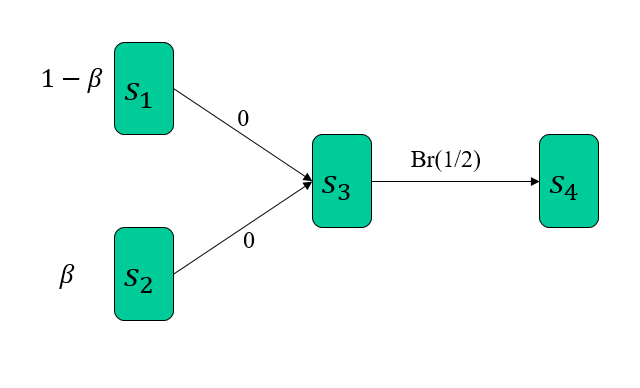
\includegraphics[width=0.5\textwidth]{figures/L7-TD-MC}\\
  \caption{Markov Reward Chain}\label{fig:L7-TD-MC}
  \end{centering}
\end{figure}


\subsection{TD: Multiple look-ahead}

The $TD(0)$ uses only the current reward and state. Given
$(\state_\ttime,\action_\ttime,\reward_\ttime,\state_{\ttime+1})$ it
updates $\Delta_\ttime=R^{(1)}_\ttime(\state_\ttime) -
\widehat{V}(\state_\ttime)$ where $R^{(1)}_\ttime(\state_\ttime)=
\reward_\ttime +\discount \widehat{V}(\state_{\ttime+1})$. We can
also consider a two step look-ahead as follows. Given
$(\state_\ttime,\action_\ttime,\reward_\ttime,\state_{\ttime+1},\action_{\ttime+1},\reward_{\ttime+1},\state_{\ttime+2})$
we can update using
$\Delta^{(2)}_\ttime=R^{(2)}_\ttime(\state_\ttime) -
\widehat{V}(\state_\ttime)$ where $R^{(2)}_\ttime(\state_\ttime)=
\reward_\ttime+\discount \reward_{\ttime+1} +\discount^2
\widehat{V}(\state_{\ttime+2})$. Using the same logic, we have that
this is a temporal difference that uses a two time steps.

We can generalize this to any $n$-step look-ahead and define
$R^{(n)}_\ttime(\state_\ttime)= \sum_{i=0}^{n-1} \discount^i
\reward_{\ttime+i}+\discount^n \widehat{V}(\state_{\ttime+n})$ and
updates $\Delta^{(n)}_\ttime=R^{(n)}_\ttime(\state_\ttime) -
\widehat{V}(\state_\ttime)$.

We can relate the $\Delta^{(n)}_\ttime$ to the $\Delta_\ttime$ as
follows:
\[
\Delta^{(n)}_\ttime=\sum_{i=0}^{n-1} \discount^i \Delta_{\ttime+i}
\]
This follows since
\[
\sum_{i=0}^{n-1} \discount^i \Delta_{\ttime+i}=\sum_{i=0}^{n-1}
\discount^i \reward_{\ttime+i}+ \sum_{i=0}^{n-1} \discount^{i+1}
\widehat{V}(\state_{\ttime+i+1})- \sum_{i=0}^{n-1} \discount^{i}
\widehat{V}(\state_{\ttime+i})=\sum_{i=0}^{n-1} \discount^i
\reward_{\ttime+i}+\discount^n
\widehat{V}(\state_{\ttime+n})-\widehat{V}(\state_\ttime)
\]

Using the $n$-step look-ahead we have
$\widehat{V}(\state_\ttime)=\widehat{V}(\state_\ttime)+\alpha_\ttime
\Delta^{(n)}_\ttime$ where
$\Delta^{(n)}_\ttime=R^{(n)}_\ttime(\state_\ttime)-\widehat{V}(\state_\ttime)$.
We can view $R^{(n)}_\ttime$ as an operator over $V$, and this operator is
%Note that the operator $R^{(n)}_\ttime$ is
$\discount^n$-contracting, namely
\[
\| R^{(n)}_\ttime(V_1)-R^{(n)}_\ttime(V_2)\|_\infty \leq \discount^n
\|V_1-V_2\|_\infty
\]

We can use any parameter $n$ for the $n$-step look-ahead. If the
episode ends before step $n$ we can pad it with rewards zero. This
implies that for $n=\infty$ we have that $n$-step look-ahead is
simply the Monte-Carlo estimate. However, we need to select some
parameter $n$. An alternative idea is to simply average over the
possible parameters $n$. One simple way to average is to use
exponential averaging with a parameter $\lambda\in(0,1)$. This
implies that the weight of each parameter $n$ is
$(1-\lambda)\lambda^{n-1}$.

This leads us to the $TD(\lambda)$ update:
\[
\widehat{V}(\state_\ttime)=\widehat{V}(\state_\ttime)+\alpha_\ttime(1-\lambda)\sum_{n=1}^\infty
\lambda^{n-1}\Delta^{(n)}_\ttime
\]

\noindent{\bf Remark:} While both $\discount$ and $\lambda$ are used
to generate exponential decaying values, their goal is very
different. The discount parameter $\discount$ defines the objective
of the MDP, the goal that we like to maximize. The exponential
averaging parameter $\lambda$ is used by the learning algorithm to average over the different
look-ahead parameters, and is selected to optimize the convergence.

%In the slides there is an example of a random walk and its
%convergence taken from \cite{SuttonB98}.

The above describes the forward view of $TD(\lambda)$, where we
average over future rewards. If we will try to implement it in a
strict way this will lead us to wait until the end of the episode,
since we will need to first observe all the rewards. Fortunately,
there is an equivalent form of the $TD(\lambda)$ which uses a {\em
backward view}. The backward view updates at each time step, using
an incomplete information. At the end of the episode, the updates of
the forward and backward updates will be the same.

The basic idea of the backward view is the following. Fix a time
$\ttime$ and a state $\state=\state_\ttime$. We have at time
$\ttime$ a temporal difference $\Delta_\ttime= \reward_\ttime
+\discount V_\ttime(\state_{\ttime+1})-V_\ttime(\state_\ttime)$.
Consider how this $\Delta_\ttime$ affects all the previous times
$\tau<\ttime$ where $\state_\tau=\state=\state_\ttime$. The influence is
exactly $(\discount\lambda)^{\ttime-\tau}\Delta_\ttime$. This implies
that for every such $\tau$ we can do the desired update, however, we
can aggregate all those updates to a single update. Let,
\[
e_\ttime(\state)=\sum_{\tau\leq \ttime: \state_\tau=\state}
(\discount\lambda)^{\ttime-\tau} = \sum_{\tau=1}^\ttime
(\discount\lambda)^{\ttime-\tau}I(\state_\tau=\state)
\]
The above $e_\ttime(\state)$ defines the {\em eligibility trace} and
we can compute it online using
\[
e_\ttime(\state)=\discount\lambda
e_{\ttime-1}(\state)+I(\state=\state_\ttime)
\]
which result in the update
\[
\widehat{V}_{\ttime+1}(\state)=\widehat{V}_\ttime(\state)+\alpha_\ttime
e_\ttime(\state)\Delta_\ttime
\]
Note that for $TD(0)$ we have that $\lambda=0$ and the eligibility
trace becomes $e_\ttime(\state)=I(\state=\state_\ttime)$. This
implies that we update only $\state_\ttime$ and
$\widehat{V}_{\ttime+1}(\state_\ttime)=\widehat{V}_\ttime(\state_\ttime)+\alpha_\ttime
\Delta_\ttime$.

\paragraph{$TD(\lambda)$ algorithm}\ \\

 -- Initialization: Set $\widehat{V}(\state)=0$ (or any other value), and
 $e_0(\state)=0$.

 -- Update: observe $(\state_\ttime,\action_\ttime,\reward_\ttime,\state_{\ttime+1})$ and set
\begin{align*}
\Delta_\ttime &= \reward_\ttime +\discount \widehat{V}_\ttime(\state_{\ttime+1})-\widehat{V}(\state_\ttime)\\
e_\ttime(\state) &= \discount\lambda e_{\ttime-1}(\state)+I(\state=\state_\ttime)\\
\widehat{V}_{\ttime+1}(\state) &=
\widehat{V}_\ttime(\state)+\alpha_\ttime e_\ttime
(\state)\Delta_\ttime
\end{align*}

 To summarize, the
benefit of $TD(\lambda)$ is that it interpolates between $TD(0)$ and
Monte-carlo updates, and many times achieves superior performance to
both.
%
Similar to $TD(0)$, also  $TD(\lambda)$ can be written as a
stochastic approximation iterative algorithm, and one can derive its
convergence.
%
In the next section we show the equivalence of the forward and
backward $TD(\lambda)$ updates.
%

\subsection{The equivalence of the forward and backward view}

We would like to show that indeed the forward and backward view
result in the same overall update.

For the forward view we define the updates to be
$\Delta^F_\ttime(\state)=\alpha(R^\lambda_\ttime-V_\ttime(\state))$,
where $R^\lambda_\ttime=(1-\lambda)\sum_{n=1}^\infty
\lambda^{n-1}R_\ttime^{(n)}$. Equivalently,
$\Delta^F_\ttime(\state)=\alpha (1-\lambda)\sum_{n=1}^\infty
\Delta_\ttime ^{(n)}$.


For the backward view we define the updates to be
$\Delta^B_\ttime(\state)=\alpha\Delta_\ttime e_\ttime(\state)$,
where the eligibility trace is
$e_\ttime(\state)=\sum_{k=0}^\ttime(\lambda\discount)^{\ttime-k}I(\state=\state_k)$.

\begin{theorem}
%For any trajectory of length $T$ we have
\[
\sum_{\ttime=0}^{\infty} \Delta V ^B_\ttime
(\state)=\sum_{\ttime=0}^{\infty} \Delta V_\ttime^F(\state)
I(\state_\ttime=\state)
\]
\end{theorem}

\begin{proof}
Consider the sum of the forward updates for state $\state$:
\begin{align}
\sum_{\ttime=0}^{\infty } \Delta \Value^F_\ttime (\state)&=
\sum_{\ttime=0}^{\infty} \alpha
(1-\lambda) \sum_{n=\ttime}^{\infty} \lambda^{n-\ttime}\Delta_\ttime^{(n)} I(\state=\state_\ttime)\nonumber\\
%
&= \sum_{\ttime=0}^{\infty}  \alpha
(1-\lambda) \sum_{n=\ttime}^{\infty} \lambda^{n-\ttime}\sum_{i=0}^n \discount^i \Delta_{\ttime+i} I(\state=\state_\ttime)\nonumber\\
%
&=\sum_{\ttime=0}^\infty \sum_{n=0}^\infty \sum_{k=\ttime}^n \alpha
(1-\lambda)
\lambda^{n-k}\lambda^{k-\ttime}\discount^{k-\ttime}\Delta_k I(\state=\state_\ttime)\nonumber\\
%
&=\sum_{\ttime=0}^\infty \sum_{k=\ttime}^\infty \alpha
(\discount\lambda)^{k-\ttime}\Delta_k I(\state=\state_\ttime) \sum_{i=0}^\infty (1-\lambda)\lambda^{i}\nonumber\\
%
&= \sum_{\ttime=0}^\infty \sum_{k=\ttime}^\infty \alpha
(\discount\lambda)^{k-\ttime} \Delta_k(\state)
I(\state=\state_\ttime) \label{eq:TD-F}
\end{align}
where the first identity is the definition, the second identity
follows since $\Delta_\ttime^{(n)}=\sum_{i=0}^n\discount^i
\Delta_{\ttime+i}$, in the third identity we substitute $k$ for
$\ttime+i$ and sum over $n$, $k$ and $\ttime$, in the forth identity we
substitute $i$ for $n-k$ and isolate the terms that depend on $i$,
and in the last identity we note that $\sum_{i=0}^\infty
(1-\lambda)\lambda^{i}=1$.

For the backward view for state $\state$ we have
\begin{align}
\sum_{\ttime=0}^{\infty } \Delta \Value^B_\ttime (\state)&=\sum_{\ttime=0}^{\infty} \alpha
\Delta_\ttime(\state) e_{\ttime}(\state)\\
\sum_{\ttime=0}^{\infty} \alpha
\Delta_\ttime(\state) \sum_{k=0}^\ttime (\discount\lambda)^{\ttime-k} I(\state=\state_\ttime)\nonumber\\
&= \sum_{k=0}^\infty \sum_{\ttime=k}^\infty \alpha
(\discount\lambda)^{\ttime-k}\Delta_\ttime(\state)I(\state=\state_\ttime)
\label{eq:TD-B}
\end{align}

Note that if we interchange $k$ and $\ttime$ in Eq. (\ref{eq:TD-F})
and in Eq. (\ref{eq:TD-B}), then we have the identical expressions.
\end{proof}

\subsection{$SARSA(\lambda)$}

We can use the idea of eligibility traces also in other algorithms,
such as SARSA. Recall that given
$(\state_\ttime,\action_\ttime,\reward_\ttime,\state_{\ttime+1},\action_{\ttime+1})$
the update of SARSA is
\[
\reward_\ttime+\discount
Q_\ttime(\state_{\ttime+1},\action_{\ttime+1})-Q_\ttime(\state_\ttime,\action_\ttime)
\]
Similarly, we can define an $n$-step look-ahead
$q^{(n)}_\ttime=\sum_{i=0}^{n-1}\discount^i \reward_{\ttime+i}
+\discount^n Q_\ttime(\state_{\ttime+n},\action_{\ttime+n})$ and set
$Q_{\ttime+1}(\state_\ttime,\action_\ttime)=Q_\ttime(\state_\ttime,\action_\ttime)+\alpha_\ttime
(q^{(n)}_\ttime-Q_\ttime(\state_\ttime,\action_\ttime))$.

We can now define $SARSA(\lambda)$ using exponential averaging with
parameter $\lambda$. Namely, we define
$q^\lambda_\ttime=(1-\lambda)\sum_{n=1}^\infty
\lambda^{n-1}q^{(n)}_{\ttime}$. This makes the forward view of
$SARSA(\lambda)$ to be
$Q_{\ttime+1}(\state_\ttime,\action_\ttime)=Q_\ttime(\state_\ttime,\action_\ttime)+\alpha_\ttime
(q^{\lambda}_\ttime-Q_\ttime(\state_\ttime,\action_\ttime))$.


Similar to $TD(\lambda)$, we can define a backward view using
eligibility traces:
\begin{align*}
e_0(\state,\action)&=0\\
e_\ttime(\state,\action)&=\discount\lambda
e_{\ttime-1}(\state,\action)+ I(\state=\state_\ttime,
a=\action_\ttime)
\end{align*}
For the update we have
\begin{align*}
\Delta_\ttime&= \reward_\ttime +\discount Q_\ttime(\state_{\ttime+1},\action_{\ttime+1})-Q_\ttime(\state_\ttime,\action_\ttime)\\
Q_{\ttime+1}(\state,\action)&=Q_{\ttime}(\state,\action)+\alpha_\ttime
e_\ttime(\state,\action)\Delta_\ttime
\end{align*}

\section{Miscellaneous}

\subsection{Importance Sampling}

Importance sapling is a simple general technique to estimate the
mean with respect to a given distribution, while sampling from a
different distribution. To be specific, let $Q$ be the sampling
distribution and $P$ the evaluation distribution. The basic idea is
the following
\[
E_{x\sim P}[f(x)]=\sum_x P(x)f(x)=\sum_x Q(x)\frac{P(x)}{Q(x)}
f(x)=E_{x\sim Q} [\frac{P(x)}{Q(x)}f(x)]
\]
This implies that given a sample $\{x_1, \ldots , x_m\}$ from $Q$,
we can estimate $E_{x\sim P}[f(x)]$ using $\sum_{i=1}^m
\frac{P(x_i)}{Q(x_i)}f(x_i)$.

The importance sampling gives an unbiased estimator, but the
variance of the estimator might be huge, since it depends on
$P(x)/Q(x)$.

We would like to apply the idea of importance sampling to learning
in MDPs. Assume that there is a policy $\policy$ that selects the
actions, and there is a policy $\rho$ that we would like to
evaluate. For the importance sampling, given a trajectory, we need
to take the ratio of probabilities under $\rho$ and $\policy$.
\[
\frac{\rho(\state_1,\action_1,\reward_1,
\ldots,\state_{T},\action_{T},\reward_T,\state_{T+1})}{\policy(\state_1,\action_1,\reward_1,
\ldots,\state_{T},\action_{T},\reward_T,\state_{T+1})}=\prod_{\ttime=1}^T
\frac{\rho(a_\ttime|\state_\ttime)}{\policy(a_\ttime|\state_\ttime)}
\]
where the equality follows since the reward and transition
probabilities are identical, and cancel.

For Monte-Carlo, the estimates would be
\[
G^{\rho/\policy}=\prod_{\ttime=1}^T
\frac{\rho(\action_\ttime|\state_\ttime)}{\policy(\action_\ttime|\state_\ttime)}
(\sum_{\ttime=1}^T \reward_\ttime)
\]
and we have
\[
\widehat{V}^\rho (\state_1) = \widehat{V}^\rho(\state_1) +\alpha(
G^{\rho/\policy}- \widehat{V}^\rho(\state_1))
\]
This updates might be huge, since we are multiplying the ratios of
many small numbers.

For the $TD(0)$ the updates will be
\[
\Delta^{\rho/\policy}_\ttime
=\frac{\rho(\action_\ttime|\state_\ttime)}{\policy(\action_\ttime|\state_\ttime)}\reward_\ttime
+\discount \widehat{V}(\state_{\ttime+1})-\widehat{V}(\state_\ttime)
\]
and we have
\[
\widehat{V}^\rho (\state_1) = \widehat{V}^\rho(\state_1) +\alpha(
\Delta^{\rho/\policy}_\ttime- \widehat{V}^\rho(\state_1))
\]
This update is much more stable, since we have only one factor
multiplying the observed reward.


\subsection{Actor-critic methodology}


Actor-critic gives a general methodology of building reinforcement
learning algorithms. It is composed from an actor, that selects the
actions, and a critic, that learns the value function. The actor
observes the current state, and the value function, and selects an
action. The critic, observes the current state (and action) and
reward and outputs a value function. See
Figure~\ref{fig:L7-Actor-Critic}.

\begin{figure}
  % Requires \usepackage{graphicx}
  \begin{centering}
  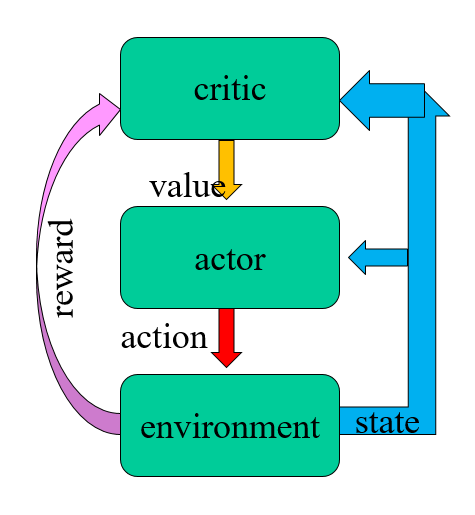
\includegraphics[width=0.5\textwidth]{figures/L7-Actor-Critic}
  \caption{The situated agent}\label{fig:L7-Actor-Critic}
  \end{centering}
\end{figure}





\section{Bibliography Remarks}

The $Q$-learning outline of the asymptotic convergence and the step
size analysis follows \cite{Even-DarM03}.

Expected SARSA was presented in \cite{SeijenHWW09}

The comparison of the {\tt First Visit} and {\tt Every Visit} is
based on \cite{SinghS96}.

Part of the outline borrows from David Silver class notes and the
the book of Sutton and Barto \cite{SuttonB98}.


The presentation of the TD algorithms follows the book of Sutton and
Barto \cite{SuttonB98}.
